
\chapter{Transmissão dos dados em série}\label{chap:chap4}

Este capítulo aborda o trabalho realizado na segunda parte do projeto, tal como definido em ~\ref{sec:descrição_objetivos}. Esta parte do projeto consiste em transmitir em paralelo para o transmissor GTX existente na FPGA VC7203 que ,através da sua arquitetura, serializa os dados e envia-os através de um cabo físico. Esse mesmo cabo conectado ao recetor GTX irá deserializar para que sejam convertidos novamente para dados em paralelo.

Este processo de serialização e deserialização exige muitos cuidados e aplicações de determinados métodos que permitam manter a integridade do sinal durante a transmissão do mesmo, já como explicado em no capítulo 2 em \ref{serial_theory}. Todavia nesse mesmo capítulo, em \ref{sub:arqGTX} foi já abordado que FPGA VC7203 possui entradas e saídas de alta velocidade com arquiteturas que possuem blocos que permitem a implementação destes mecanismos. Na imagem \ref{fig:gtx_geral_arq} da página \pageref{fig:gtx_geral_arq} visualiza-se uma arquitetura geral dos transcetores, mas estes serão descritos com mais detalhe neste capítulo.

Este capítulo começa por abordar as arquiteturas transmissora e recetora com mais detalhe, quais as características que são vantajosas a este projeto e ainda analisar as vantagens de desvantagens de algumas para poder fazer uma melhor escolha para o projeto. De seguida serão contempladas as arquiteturas desenvolvidas e explicadas todas as decisões no seu desenvolvimento.

\section{Transmissor} \label{sec:tx_gtx}

Na figura \ref{fig:gtx_tx_arq} da página \pageref{fig:gtx_tx_arq} visualiza-se a arquitetura do transmissor GTX. Assim como já foi mencionado, esta arquitetura possui muitos blocos com diferentes funções que permitem manter a integridade do sinal durante uma transmissão, pelo menos, daquilo que se pode fazer do lado do transmissor.
\begin{figure}[h!]
	\begin{center}
		\leavevmode
		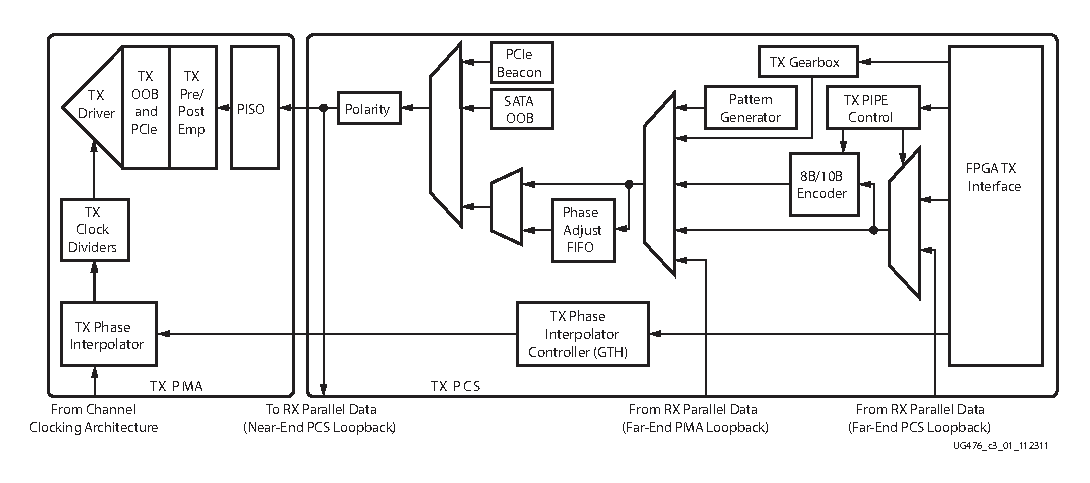
\includegraphics[width=1.0\textwidth]{tx_gtx_arq}
		\caption[Arquitetura do transmissor GTX]{Arquitetura do transmissor GTX (retirada de \cite{R011})}
		\label{fig:gtx_tx_arq}
	\end{center}
\end{figure}

Os blocos mais relevantes para o funcionamento do projeto passam de seguida a ser descritos nas próxima subsecções para que se possa entender mais facilmente as arquiteturas desenvolvidas quando estas forem apresentadas.

\subsection{Interface com a FPGA} \label{subch:tx_interface}

Na imagem \ref{fig:gtx_tx_arq} este bloco tem o nome de "\textit{FPGA TX Interface}" e é o bloco por onde entram os dados em paralelo provenientes da FPGA que se pretendem serializar. Segundo \cite{R011}, o tamanho desta interface depende de vários fatores internos, como por exemplo, o tamanho interno que os dados terão (pode estar dependente da utilização de codificação) e ainda o tamanho do \textit{datapath} que se escolhe usar.

%%Tamanho das interfaces
Para se perceber melhor como o tamanho da porta desta interface pode variar é apresentada a table \ref{table:tx_interface} na página \pageref{table:tx_interface} que expõe os casos possíveis.


\begin{table}[h!]
	\centering
	\resizebox{\textwidth}{!}{%
		\begin{tabular}{rlll}
			\hline
			\multicolumn{1}{c}{\textbf{Codificação 8B/10B}} & \multicolumn{1}{c}{\textbf{Tamanho do \textit{datapath}}} & \multicolumn{1}{c}{\textbf{Tamanho Interno}} & \multicolumn{1}{c}{\textbf{Interface com a FPGA}} \\ \hline
			\multicolumn{1}{r|}{Sim}                        & 0 (2 byte)                                       & 20                                           & 16                                                \\
			\multicolumn{1}{r|}{Sim}                        & 0 (2 byte)                                       & 20                                           & 32                                                \\
			\multicolumn{1}{r|}{Sim}                        & 1 (4 byte)                                       & 40                                           & 32                                                \\
			\multicolumn{1}{r|}{Sim}                        & 1 (4 byte)                                       & 40                                           & 64                                                \\
			\multicolumn{1}{r|}{Não}                        & 0 (2 byte)                                       & 16                                           & 16                                                \\
			\multicolumn{1}{r|}{Não}                        & 0 (2 byte)                                       & 20                                           & 20                                                \\
			\multicolumn{1}{r|}{Não}                        & 0 (2 byte)                                       & 16                                           & 32                                                \\
			\multicolumn{1}{r|}{Não}                        & 1 (4 byte)                                       & 32                                           & 32                                                \\
			\multicolumn{1}{r|}{Não}                        & 0 (2 byte)                                       & 20                                           & 40                                                \\
			\multicolumn{1}{r|}{Não}                        & 1 (4 byte)                                       & 40                                           & 40                                                \\
			\multicolumn{1}{r|}{Não}                        & 1 (4 byte)                                       & 32                                           & 64                                                \\
			\multicolumn{1}{r|}{Não}                        & 1 (4 byte)                                       & 40                                           & 80                                                \\ \hline
		\end{tabular}%
	}
	\caption[Tamanhos possíveis para a interface da FPGA com o GTX transmissor]{Tamanhos possíveis para a interface da FPGA com o GTX transmissor (adaptada de \cite{R011})}
	\label{table:tx_interface}
\end{table}

Os diferentes tamanhos que a porta da interface pode tomar estão apresentados na última coluna da tabela tendo em conta que quando é implementada uma codificação então estes apenas podem variar entre 16, 32 ou 64. Todavia quando não há codificação, então o tamanho desta porta pode ser os valores anteriormente referidos ou então até mesmo 20,40 ou 80. De notar que quando não há codificação e o tamanho da porta é 16, 32 ou 64 existe a possibilidade de extender esses valores (caso se pretenda) para 20, 40 e 80 respetivamente. No entanto, tal não será abordado dado que não é importante para o projeto. 

Os valores do tamanho interno do \textit{datapath} podem variar entre 2 e 4 bytes, contudo é necessário tomar em atenção que quando um \textit{datapath} de um determinado tamanho não chega para o número de bits à entrada então é necessário utilizar dois. Mas isto será abordado mais à frente nesta subsecção. 

%%Relógios que saem e para que servem
Os dados em paralelo entram neste bloco a uma determinada cadência bem definida : ao flanco positivo do sinal de relógio \textit{TXUSRCLK2}. Este sinal de relógio é o sinal de sincronização entre os dados provenientes da FPGA com o transmissor, no entanto é também necessário outro sinal de relógio para a lógica interna PCS do transmissor : \textit{TXUSRCLK}. De recordar que a lógica interna PCS trabalha com os dados em paralelo ainda e portanto o valor deste sinal de relógio vai depender não só da cadência a que os dados em paralelo (\textit{TXUSRCLK2}) entram no transmissor mas também do \textit{datapath} escolhido.

Por um lado, o sinal de relógio \textit{TXUSRCLK2} é o principal sinal de sincronização entre a lógica da FPGA e a lógica do transmissor, por outro o sinal de relógio \textit{TXUSRCLK} é a cadência determinista dos dados em paralelo no bloco PCS, e por isso existe uma relação entre estes dois sinais muito bem definida que passa a ser apresentada na tabela \ref{table:freq_tx} na página \pageref{table:freq_tx}.

\begin{table}[h!]
	\centering
	\resizebox{\textwidth}{!}{%
		\begin{tabular}{lll}
			\hline
			\multicolumn{1}{c}{\textbf{Tamanho na Interface}} & \multicolumn{1}{c}{\textbf{Tamanho do \textit{datapath}}} & \multicolumn{1}{c}{\textbf{Relação entre os sinais de relógio}} \\ \hline
			16, 20 (bits)                                     & 0 (2 byte)                                       & $F_{TXUSRCLK} = F_{TXUSRCLK2}  $                                    \\
			32, 40 (bits)                                     & 0 (2 byte)                                       & $F_{TXUSRCLK} = F_{TXUSRCLK2} * 2$                                  \\
			32, 40 (bits)                                     & 1 (4 byte)                                       & $F_{TXUSRCLK} = F_{TXUSRCLK2} $                                      \\
			64, 80 (bits)                                     & 1 (4 byte)                                       & $F_{TXUSRCLK} = F_{TXUSRCLK2} * 2$                                  \\ \hline
		\end{tabular}%
	}
	\caption[Relação entre as frequências dos sinais de relógio \textit{TXUSRCLK2} e \textit{TXUSRCLK}]{Relação entre as frequências dos sinais de relógio \textit{TXUSRCLK2} e \textit{TXUSRCLK} (adaptada de \cite{R011})}
	\label{table:freq_tx}
\end{table}


%Explicar que se pode obter uma estimativa da velocidade de transmissão de acordo com aquela equação
Segundo \cite{R011}, sabendo estas relações entre os sinais de relógio, o tamanho da porta na interface do transmissor e o tamanho do \textit{datapath} usado é possível obter a velocidade de transmissão do dados em série através da equação apresentada em \ref{eq:lineRate} na página \pageref{eq:lineRate}.

\begin{equation} \label{eq:lineRate}
Line\ Rate = F_{TXUSRCLK}*(Internal\ Datapath\ Width)
\end{equation}


%Explicar pq e que tem frequências diferentes visto que sao os dois para sinais em paralelo
Para que se perceba a diferença entre estas frequências é agora apresentado um caso em concreto que é utilizado neste projeto: pretende-se na entrada do transmissor obter 40 bits em paralelo, ou seja, ter uma porta com uma largura de 40 bits, e que estes dados sejam amostrados a uma frequência de 148,5 MHz ($F_{TXUSRCLK2} = 148,5\ MHz$). Assim sendo, existem agora duas hipóteses: a utilização de um \textit{datapath} de 2 byte ou 4 byte.

Se se optar pela utilização de um \textit{datapath} de 4 byte então está-se perante a opção a), ilustrada na imagem \ref{fig:exemplo_datapaths} da página \pageref{fig:exemplo_datapaths}, em que o sinal de amostragem à entrada é de 148,5 MHz ($F_{TXUSRCLK2} = 148,5\ MHz$) e o sinal de lógica do bloco PCS também é 148,5 MHz ($F_{TXUSRCLK} = 148,5\ MHz$), tal como ilustrado na figura. Neste caso a largura do sinal interno é de 40 bits o que, segundo a equação \ref{eq:lineRate}, perfaz uma taxa de saída do sinal serializado de $5,94\ Gb/s$.

Se por outro lado, se optar por um \textit{datapath} interno de 2 byte, então serão necessários 2 \textit{datapaths}, tal como ilustra o caso b) da figura \ref{fig:exemplo_datapaths}. Isto implica que a taxa de amostragem nesses sejam o dobro da cadência de entrada dos sinais na interface com transmissor. Assim, mantém-se uma frequência de amostragem à entrada do transmissor de $F_{TXUSRCLK2} = 148,5\ MHz$ e uma frequência do sinal de relógio de cada bloco PCS de $F_{TXUSRCLK} = 297\ MHz$. Ou seja, a largura interna de cada datapath é de 20 bits e por isso a taxa de saída do sinal serializado será igual a $5,94\ Gb/s$, segundo a equação \ref{eq:lineRate}.

\begin{figure}[h!]
 	\begin{center}
 		\leavevmode
 		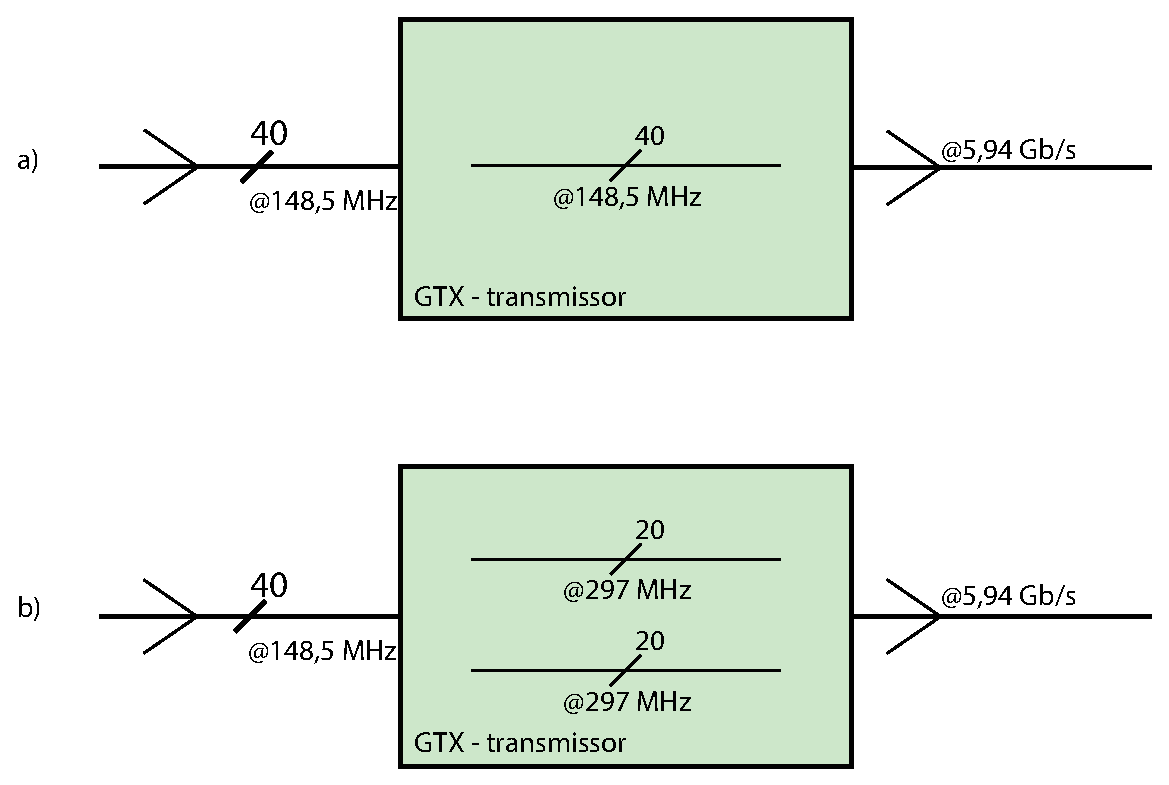
\includegraphics[width=0.75\textwidth]{exemplo_datapath}
 		\caption[Exemplo simplificado de transmissão com diferentes usos de \textit{datapath}]{Exemplo simplificado de transmissão com diferentes usos de \textit{datapath}}
 		\label{fig:exemplo_datapaths}
 	\end{center}
 \end{figure}

%%Concluir como se geram estes sinais
Estes dois sinais de relógio são gerados neste bloco e colocados nas saídas do mesmo para que na FPGA possa ser desenvolvida uma arquitetura que leia os sinais em paralelo para o transmissor à cadência de \textit{TXUSRCLK2}. Estes estão alinhados pelo flanco positivo dos mesmos ainda que tenham frequências diferentes. Ambos são gerados com base no sinal de relógio de referência, segundo \cite{R011} e \cite{R022}, através de multiplicadores ou divisores caso possuam frequências diferentes.


\subsection{Codificador 8B/10B}

Este bloco permite que os sinais em paralelo sejam codificados de 8 bits para 10 bits quando está ativo. Por outras palavras, através da codificação extende os sinais de entrada de 16 bits para 20 bits, os sinais de 32 bits para 40 bits e os sinais de 64 bits para 80 bits. É de notar que apesar de ser vantajosa a utilização de codificação num protocolo de transmissão em série, que a ativação deste bloco aumenta a latência do transmissor, tal como é de esperar.

As características deste tipo de codificação, as suas vantagens e importância foram já abordadas na subsecção com o título "Codificação dos sinais e sua importância" em \ref{subsub:cod_impor} no capítulo \ref{chap:chap2}.

%\subsection{Gerador de padrões pseudo-aleatórios}
%
%A geração de sequência pseudo-aleatórias é bastante utilizada em sistemas de telecomunicações para testar a integridade do sinal de ligações de grande velocidade, segundo \cite{R011}. Apesar de estas mesmas sequências parecerem aleatórias à primeira vista, na realidade apresentam determinadas características que são utilizadas para medir a qualidade da ligação. Este bloco do transmissor é responsável por esta ação. 

\subsection{Interface entre os diferentes domínios de sinal de relógio do transmissor} \label{subsub:tx_buffer}

Já foi referido anteriormente que para o correto funcionamento do transmissor GTX opera com pelo menos dois sinais de relógio diferentes : TXUSRCLK and TXUSRCLK2. O segundo é o sinal de relógio de sincronização principal entre os dados provenientes da FPGA e o transmissor, e o primeiro é o sinal de relógio utilizado para a lógica do bloco PCS.

Contudo, o bloco PCS utiliza dois sinais de relógio internamente para o seu correto funcionamento: TXUSRCLK (como já foi mencionado) e ainda XCLK (sinal de relógio dos dados em paralelo do bloco PMA). A figura \ref{fig:clk_domains_tx} ilustra os diferentes domínios de relógio presentes no transmissor GTX.

\begin{figure}[h!]
	\begin{center}
		\leavevmode
		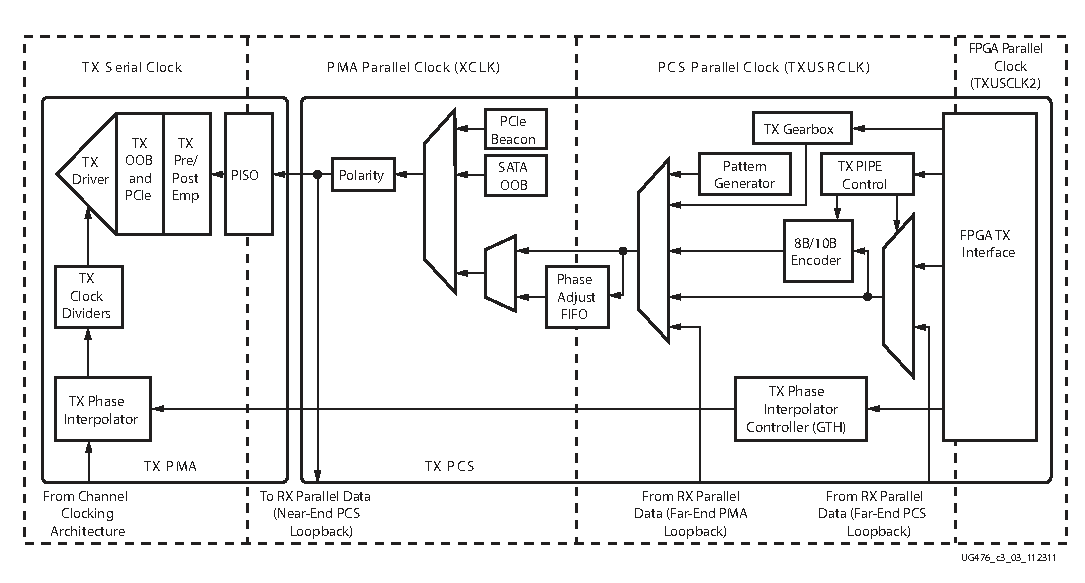
\includegraphics[width=1.0\textwidth]{clk_domain_cross_gtx_tx}
		\caption[Diferentes domínios de sinal de relógio do transmissor]{Diferentes domínios de sinal de relógio do transmissor (retirada de \cite{R011})}
		\label{fig:clk_domains_tx}
	\end{center}
\end{figure}

Quando os dados se cruzam entre os domínios TXUSRCLK e XCLK é necessário que para além de terem frequências semelhantes, as diferenças de fase que possam existir estejam resolvidas, e por isso existem dois blocos responsáveis por tal que apresentam os seus prós e contras: \textit{buffer} ou bloco de alinhamento de fase. Independentemente da escolha de um ou de outro, a utilização de um deles é obrigatória e torna-se importante conhecer as suas vantagens e desvantagens, pois tal escolha afeta o funcionamento global do sistema, segundo \cite{R011}.

Por um lado, a utilização de um \textit{buffer} é mais fácil e ainda assim é robusta, por outro o bloco de alinhamento de fase exige a utilização de mais lógica e restrições de sinais de relógio adicionais. Quando a latência se torna um ponto importante do sistema, então a utilização do \textit{buffer} deve ser posta de lado, visto que o bloco de alinhamento de fase utiliza menos registos obtendo assim uma latência menor. Por outro lado, quando se utilizam várias transmissões em transcetores diferentes à mesma velocidade, o bloco de alinhamento de fase tem a vantagem de diminuir o atraso entre as mesmas. No entanto, isto é apenas uma curiosidade visto que tal não é utilizado no projeto.

\subsection{Interface com a camada física} 
Após a serialização dos dados no bloco PISO da figura \ref{fig:gtx_tx_arq} da página \pageref{fig:gtx_tx_arq} os sinais são transmitidos para a camada física através de um \textit{driver} reconfigurável. Esta interface dispões de várias características que permitem manter a integridade do sinal, que passam de seguida a ser brevemente apresentadas:
\begin{itemize}
	\item \textbf{Sinalização Diferencial:} para diminuir eventuais interferências no sinal durante a sua transmissão no cabo físico, tal como mencionado na subsecção com o título "Sinalização Física" em \ref{subsub:sinalizacao_fisica} no capítulo \ref{chap:chap2}.
	\item \textbf{Pré-ênfase:} para de certa maneira preparar o sinal transmitido para um canal ruidoso, tal como referido na subsecção com o título "Interfaces com a camada física" em \ref{subsub:pre_enfase_equalizacao} no capítulo \ref{chap:chap2}.
	\item \textbf{Resistências de interface com o cabo calibráveis:} para que a impedância característica da linha esteja adaptada com a interface, evitando assim eventuais reflexões dos sinais, tal como mencionado em na subsecção com o título "Restrições na utilização de circuitos de serializadores e deserializadores" em \ref{subsub:restricoes_circuitos} do capítulo \ref{chap:chap2}.
\end{itemize}


\section{Recetor} \label{sec:_rx_gtx}
Na figura \ref{fig:gtx_rx_arq} na página \pageref{fig:gtx_rx_arq} é possível visualizar a arquitetura do recetor GTX. Este inclui diversos blocos que permitem a correta recuperação do sinal, sendo que o funcionamento dos principais já foram mencionados na subsecção \ref{serial_theory} do capítulo \ref{chap:chap2}, contudo passarão de seguida a ser brevemente descritos nas próximas subsecções. 

\begin{figure}[h!]
	\begin{center}
		\leavevmode
		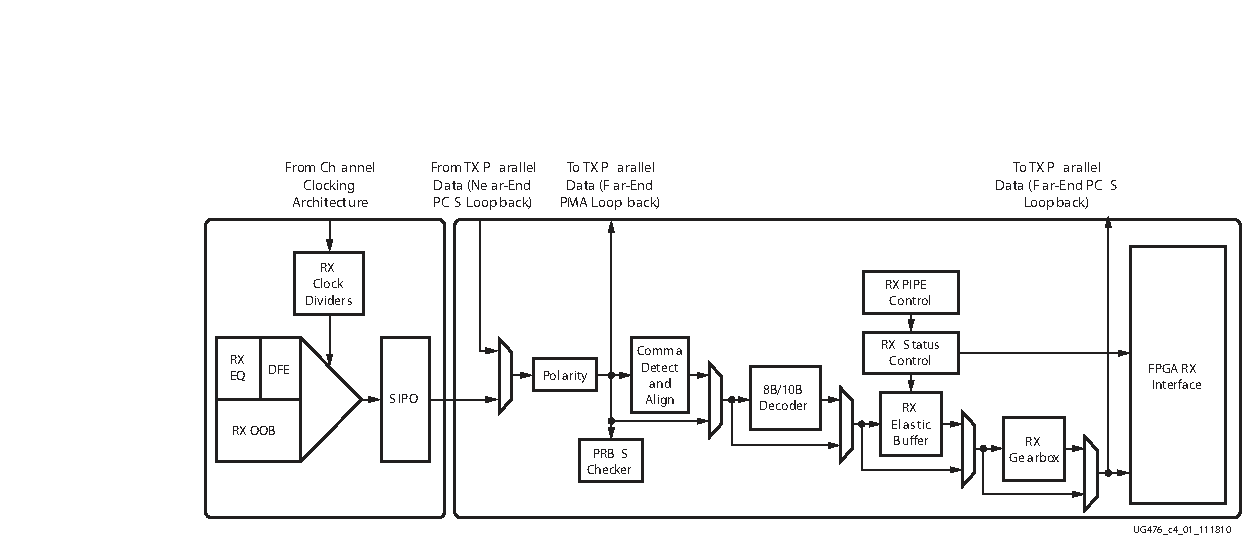
\includegraphics[width=1.0\textwidth]{rx_gtx_arq}
		\centering
		\caption[Arquitetura do recetor GTX]{Arquitetura do recetor GTX, (retirada de \cite{R011})}
		\label{fig:gtx_rx_arq}
	\end{center}
\end{figure}
	

\subsection{Interface com a camada física}

A interface o cabo físico do recetor possui duas características que se tornam importantes para a recuperação do sinal:
\begin{itemize}
	\item \textbf{Tensão de terminação configurável:} Esta característica é importante quando a referência do sinal diferencial é variável do lado do transmissor, o que permite recuperar bem diferencial do lado do transmissor.
	\item \textbf{Resistências de interface com o cabo configuráveis:} tal como acontecia do lado do transmissor, esta característica torna-se importante para que a linha de transmissão esteja adaptada ao recetor, evitando assim eventuais reflexões do sinal para a sua correta recuperação.


\end{itemize}


\subsection{Equalização} \label{subsub:rx_equalização}

Na subsecção com o nome de "Interfaces com a camada física" em \ref{subsub:pre_enfase_equalizacao} do capítulo \ref{chap:chap2} foi abordada a importância da utilização de filtros equalizadores para tentar compensar a atenuação e distorção que sinal sofre durante a sua transmissão no canal físico. O recetor GTX disponibiliza dois tipos de equalizadores adaptativos que devem ser escolhidos consoante as necessidades de consumo de potência do circuito \textit{versus} perdas do canal físico de transmissão.

Segundo \cite{R011}, para canais cujas perdas não são muito significativas e o consumo de potência torna-se uma característica crítica do circuito existe um filtro adaptativo otimizado para tal com o nome de LPM (\textit{Low-power mode}). Ainda segundo esta fonte o uso deste tipo de equalizador é recomendado para aplicações com débitos até 11,2 Gb/S de curto alcance, e com perdas por canal até 12 dB à frequência de \textit{Nyquist}.


Para canais cujas perdas tornam-se significativas existe disponível um filtro adaptativo com o nome de\textit{ Decision Feedback Equalizer} (DFE). 
%Este é um filtro que utiliza a realimentação de símbolos detetados para produzir uma estimação da saída do canal. 
Segundo \cite{R011}, este equalizador é utilizado para ligações de média distância cujas perdas do canal rondam os 8 dB ou mais à frequência de \textit{Nyquist}. Para além disso, a utilização deste tipo de equalizador traz as seguintes vantagens adicionais:
\begin{itemize}
	\item Efetua a equalização sem amplificação do ruído ou eventuais interferências.
	\item Pode também fazer correções de reflexões causadas pelas descontinuidades do canal. 
	\item É vantajosa a sua utilização quando as interferências são preocupantes.
\end{itemize}

%\textbf{Cuidados a ter na utilização deste tipo de equalizador:}
%\begin{itemize}
%	\item Este tipo de equalização deve ser cuidadosa quando não existe codificação de dados, uma vez que pode levar à não equalização ideal do sinal recebido (pois o filtro pode não se auto adaptar aos dados recebidos).
%\end{itemize}

Tendo em conta as vantagens dos dois equalizadores disponíveis no recetor GTX, verifica-se que a utilização de cada um deles pode ser utilizada em circunstâncias diferentes: numa fase inicial pode ser utilizado um equalizador DFE, apesar de gastar mais energia, contudo a utilização de um equalizador LPM reduz o consumo. Todavia, numa fase mais avançada do projeto, que envolva a inserção dos sinais em ligações longas e/ou ruidosas, faz mais sentido usar um filtro DFE adaptado para tal. 

%
%Conhecendo agora os prós e contras dos dois equalizadores disponíveis no recetor GTX conclui-se que numa fase inicial do projeto em que nao se pretende usar codificação, e uma ligação curta não faz sentido usar um equalizador DFE, mas sim um equalizador LPM. T

%\subsection{CDR - \textit{Clock And Data Recovery}}
%
%No recetor GTX, existe um bloco responsável por uma característica muito importante de um transcetor: recuperação de sinal de relógio e dados. Segundo \cite{R011}, esse circuito faz a recuperação do relógio e dos dados através do \textit{stream} de dados que recebe. A figura \ref{fig:cdr_arq} da página \pageref{fig:cdr_arq} ilustra esse mesmo bloco.
%
%\begin{figure}[h!]
%	\begin{center}
%		\leavevmode
%		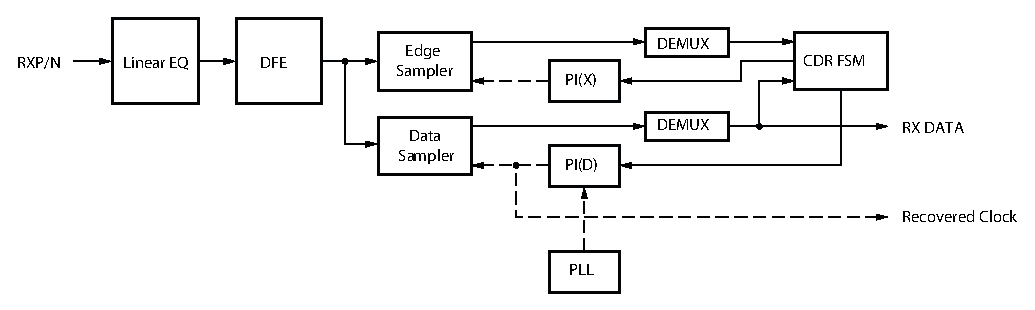
\includegraphics[width=1.0\textwidth]{cdr_arq_vet}
%		\caption{Arquitetura do circuito de recuperação de sinal de relógio e dados, retirada de \cite{R011}}
%		\label{fig:cdr_arq}
%	\end{center}
%\end{figure}
%
%%Os dados recebidos passam pelo equalizador e de seguida são capturados por um “\textit{data sampler}” e um “\textit{edge sampler}”. O “\textit{edge sampler}” captura a fase do sinal recebido em série quando este está na sua região de transição, enquanto que o “\textit{data sampler}” captura a fase do mesmo sinal a meio do olho dos dados, tal como ilustra a figura \ref{fig:exmple_cdr} da página \pageref{fig:exmple_cdr}.  Estas duas fases são de seguida enviadas para a máquina de estados do CDR para que esta consiga determinar a fase dos sinais que chegam e ao mesmo tempo controlar os interpoladores de fase (PIs). 
%
%
%\begin{figure}[h!]
%	\begin{center}
%		\leavevmode
%		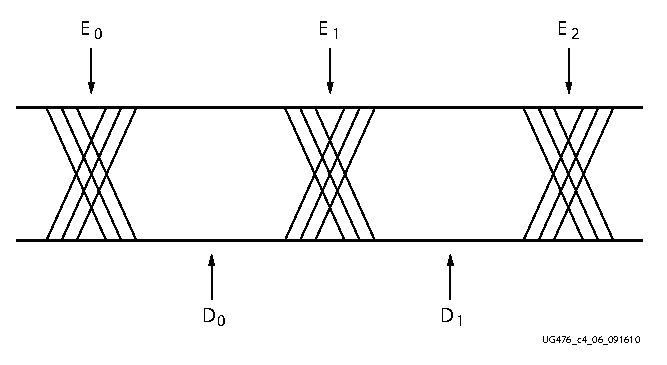
\includegraphics[width=0.5\textwidth]{exemplo_cdr}
%		\captionsetup{width=0.5\linewidth}
%		\caption{Exemplo das amostras de fase retiradas do circuito, retirada de \cite{R011}}
%		\label{fig:exmple_cdr}
%	\end{center}
%\end{figure}
%
%Na figura \ref{fig:exmple_cdr} E0, E1 e E2 correspondem ás amostras retiradas pelo "\textit{edge sampler}" e D0 e D1 às amostras retiradas pelo "\textit{data sampler}".
%A tracejado na figura \ref{fig:cdr_arq} visualiza-se o sinal de relógio recuperado com o nome de "\textit{Recovered Clock}" e os dados recuperados em série saem no sinal "\textit{RXDATA}".


\subsection{Alinhamento de Palavras} \label{subsub:align}

O bloco de alinhamento de palavras é feito antes da deserialização dos sinais, isto porque é necessário definir os limites das palavras antes destes serem convertidos para dados em paralelo. O método de alinhamento de palavras, os caracteres especiais existentes para aplicação neste método e ainda a sua importância foram já abordados na subsecção com o título "Alinhamento da transmissão" em \ref{subsub:alinhamento} no capítulo \ref{chap:chap2}.

Nesta subsecção serão abordadas as características que este bloco do recetor possui e ainda como se pode tirar partido das mesmas aquando a sua utilização. O bloco possibilita a escolha da palavra de alinhamento, pode ser uma utilizada em protocolos bastantes conhecidos, já como referido anteriormente e até pode mesmo ser a combinação de duas palavras com uma determinada máscara. Contudo, por uma questão de simplificação, o projeto utiliza apenas uma palavra de alinhamento bem conhecida que será definida quando for apresentado desenvolvimento do mesmo.

Apesar de existirem \textit{flags} disponibilizadas pelo bloco de alinhamento que indicam o estado do mesmo, o autor de \cite{R011} alerta que para uma linha de transmissão cuja taxa de débito seja superior a 5 Gb/s, o bloco pode alinhar a palavra falsamente e por isso ativar a \textit{flag} que indica que a palavra está alinhada mesmo que não estando. Isto implica que seja desenvolvido e aplicado um sistema que verifique se a palavra se encontra alinhada ou não.

%%Alinhamento Manual

Este bloco dispõe de uma opção de alinhamento manual que vem substituir o automático, o que pode ser bastante útil em casos em que o transcetor alinha falsamente uma palavra. Na imagem \ref{fig:rxslide_example} na página \pageref{fig:rxslide_example} é possível visualizar o exemplo de alinhamento manual das palavras no recetor que passa a ser brevemente descrito.

\begin{figure}[h!]
	\begin{center}
		\leavevmode
		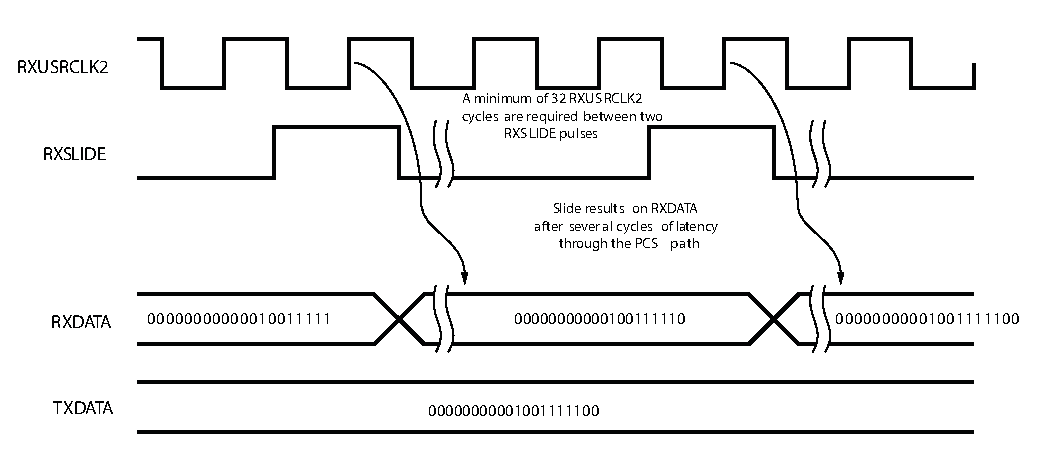
\includegraphics[width=1.0\textwidth]{rxslide_example}
		\captionsetup{width=1.0\linewidth}
		\caption[Exemplo de um alinhamento manual da palavra]{Exemplo de um alinhamento manual da palavra (retirada de \cite{R011})}
		\label{fig:rxslide_example}
	\end{center}
\end{figure}

Este processo de alinhamento manual é conhecido pelo nome de "\textit{RXSLIDE}" e é usado para mover a palavra em 1 bit. O sinal "RXSLIDE" deve estar ativo apenas um ciclo de relógio de RXUSRCLK2 e de seguida deve ser inativo. Segundo, \cite{R011} deve-se esperar pelo menos 32 ciclos de relógio para que esta operação seja realizada outra vez.  

\subsection{Descodificador 8B/10B}

Tal como no transmissor, este bloco é responsável pela descodificação 8B/10B caso esta tenha sido realizada do lado do transmissor. Esta operação é realizada depois da conversão dos dados para paralelo e é de notar que a utilização deste bloco aumenta a latência de todo o sistema.

Numa fase inicial do projeto, a utilização deste bloco (tanto do lado do transmissor como do recetor) é posta de lado no sentido de simplificar o projeto e também de diminuir a latência do sistema.   

\subsection{Interfaces entre os diferentes domínios de sinal relógio do recetor} \label{subsub:rx_buffer}

Tal como acontecia no transmissor, o recetor opera a diferentes domínios de sinal de relógio. Particularmente no bloco PCS existem dois domínios de relógio para os dados em paralelo críticos: RXUSRCLK e XCLK(o sinal de relógio dos dados em paralelo do bloco PMA). A imagem \ref{fig:dominios_rx} ilustra os diferentes domínios de relógio presentes no recetor.


\begin{figure}[h!]
	\begin{center}
		\leavevmode
		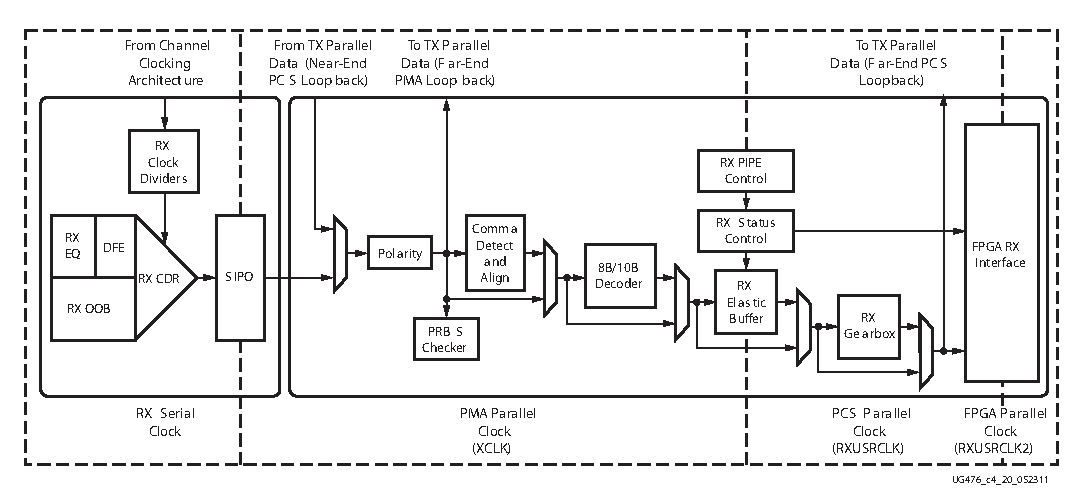
\includegraphics[width=1.0\textwidth]{dominios_rx}
		\captionsetup{width=1.0\linewidth}
		\caption[Diferentes domínios de sinal de relógio no recetor]{Diferentes domínios de sinal de relógio no recetor (retirada de \cite{R011})}
		\label{fig:dominios_rx}
	\end{center}
\end{figure}

Quando os dados são transmitidos de um domínio para o outro todas as diferenças de fase entre os sinais de relógio devem estar resolvidas e a frequência não deve variara muito, e por isso deve-se recorrer ao uso de um dos dois seguintes blocos: \textit{elastic buffer} ou bloco de alinhamento de fase. Ambos os blocos resolvem as diferenças de fase entre os dois domínios, no entanto apresentam as suas vantagens e desvantagens que serão de seguida abordadas para se concluir qual deve ser utilizado no projeto.

Por um lado, segundo \cite{R011}, o \textit{buffer} é uma estrutura robusta e de fácil operação, enquanto que o bloco de alinhamento de fase exige mais lógica e restrições relativamente às fontes de relógio. Por outro lado, o uso do \textit{buffer} implica uma latência maior visto que o bloco de alinhamento de fase foi concebido para diminuir a latência total do sistema. 

Relativamente à inicialização, o \textit{buffer} tem a capacidade de se inicializar imediatamente, enquanto que o circuito de alinhamento de fase tem de esperar que todos os sinais de relógio estabilizem para poder conseguir operar corretamente. Quanto à correção do sinal de relógio, o uso do\textit{ elastic buffer} é obrigatório, enquanto que quando se utiliza o bloco de alinhamento de palavras, este exige que a lógica de correção do sinal de relógio seja feita fora do transcetor.

Assim sendo, o uso do bloco de alinhamento torna-se útil quando a latência é um requisito crítico do sistema, todavia o uso do \textit{buffer} não requer correção de sinal de relógio externa ao transcetor o que simplifica bastante o sistema. É uma boa opção numa fase inicial do projeto utilizar um \textit{buffer} para fazer as correções de fase , pois, apesar de introduzir um pouco de latência no circuito, não exige lógica externa ao transcetor para correção do sinal de relógio.

\subsection{Interface com a FPGA}

Este é o bloco responsável pela conexão entre os dados do recetor com o resto da FPGA. Toda a lógica desenvolvida na FPGA deve receber os dados provenientes do recetor pela porta "RXDATA" lendo-os ao flanco positivo do sinal de relógio "RXUSRCLK2". O tamanho desta porta depende de vários fatores internos do recetor, tal como acontecia no transmissor,  como por exemplo se a codificação está ativa ou não e ainda qual o tamanho do \textit{datapath} usado (2 ou 4 byte). As diferentes possibilidades de larguras da porta de RXDATA assemelham-se ás da largura da porta de entrada do transmissor (TXDATA)e por isso é possível encontrá-las na tabela \ref{table:tx_interface} na página \pageref{table:tx_interface}.

Também à semelhança do transmissor existem dois sinais de relógio necessários para o correto funcionamento do recetor: RXUSRCLK e RXUSRCLK2. O segundo já foi mencionado como o sinal de relógio de sincronização entre o recetor e a lógica da FPGA, e o sinal de relógio RXUSRCLK é o sinal interno para a lógica do bloco PCS (que lida com os dados em paralelo). O valor deste relógio depende da velocidade de transmissão do canal e do tamanho interno do \textit{datapath} usados e é possível calcular o seu valor através da equação presente em \ref{eq:lineRate} na página \pageref{eq:lineRate}.

A relação entre estes dois sinais de relógio mencionados (RXUSRCLK e RXUSRCLK2), é bem definida e depende do tamanho da porta RXDATA e do tamanho do \textit{datapath} usado.  A relação entre estes dois sinais de relógio do recetor é idêntica à do transmissor e por isso é possivel encontrar essas mesmas relações na tabela \ref{table:freq_tx} na página \pageref{table:freq_tx}.

Segundo \cite{R011}, é de notar que quando é o mesmo oscilador a fornecer o sinal de relógio de referência para o transmissor e para o recetor, que para além dos sinais de relógio de saída do recetor serem gerados com base no sinal de relógio de referência, podem ainda ser usados os sinais de relógio de saída do transmissor para o recetor e vice-versa.

\section{Análise das características de transmissão}

Nesta secção são abordadas as diferentes características de transmissão possíveis de obter (velocidades de transmissão, tamanho de tramas entre outras) tendo em conta as restrições dos GTX, de maneira a otimizar a transmissão.

O projeto pode ser abordado de várias maneiras, desde a restringir a largura de banda base da transmissão até mesmo limitar o número de bits por tramas  a transmitir. No sentido de simplificar o projeto e torná-lo eficiente em termos lógicos restringiu-se a cadência de entrada dos dados no transcetor para $148,5\ MHz$, pois assim não é necessário o uso de memórias, por exemplo FIFO, para armazenar dados antes da sua entrada nos transcetores.

Com esta restrição, e para se retirar algumas conclusões relativamente à otimização de transmissão dos dados em série, efetuaram-se cálculos para as diferentes larguras na porta de dados, com a utilização de codificação ou não através da equação apresentada em \ref{eq:lineRate} da página \pageref{eq:lineRate}. Esses resultados estão apresentados na tabela \ref{table:line_rates} na página \pageref{table:line_rates}.


\begin{table}[h!]
	\centering
	\resizebox{\textwidth}{!}{%
		\begin{tabular}{@{}lllllll@{}}
			\toprule
			\textbf{\begin{tabular}[c]{@{}l@{}}Interface\\ com a \\ FPGA\end{tabular}} & \textbf{\begin{tabular}[c]{@{}l@{}}Codificação \\ 8B/10B\end{tabular}} & \textbf{\begin{tabular}[c]{@{}l@{}}Tamanho \\ do Datapath\end{tabular}} & \textbf{\begin{tabular}[c]{@{}l@{}}Tamanho \\ interno \\ do datapath\end{tabular}} & \textbf{$F_{TXUSRCLK} $} & \textbf{$F_{TXUSRCLK2}$} & \textbf{\begin{tabular}[c]{@{}l@{}}Velocidade \\ em série\end{tabular}} \\ \toprule
			\multirow{2}{*}{16}                                                        & Sim                                                                    & 2 byte                                                                  & 20                                                                                 & 148, 5 MHz             & 148, 5 MHz              & 2,97 Gb/s                                                               \\
			& Não                                                                    & 2 byte                                                                  & 16                                                                                 & 148,5 MHz              & 148,5 MHz               & 2,376 Gb/s                                                              \\ \hline
			20                                                                         & Não                                                                    & 2 byte                                                                  & 20                                                                                 & 148,5 MHz              & 148,5 MHz               & 2,97 Gb/s                                                               \\ \hline
			\multirow{4}{*}{32}                                                        & Sim                                                                    & 2 byte                                                                  & 20                                                                                 & 297 MHz                & 148,5 MHz               & 5,94 Gb/s                                                               \\
			& Não                                                                    & 2 byte                                                                  & 16                                                                                 & 297 MHz                & 148,5 MHz               & 4,752 Gb/s                                                              \\
			& Sim                                                                    & 4 byte                                                                  & 40                                                                                 & 148,5 MHz              & 148,5 MHz               & 5,94 Gb/s                                                               \\
			& Não                                                                    & 4 byte                                                                  & 32                                                                                 & 148,5 MHz              & 148,5 MHz               & 4,752 Gb/s                                                              \\ \hline
			\multirow{2}{*}{40}                                                        & Não                                                                    & 2 byte                                                                  & 20                                                                                 & 297 MHz                & 148,5 MHz               & 5,94 Gb/s                                                               \\
			& Não                                                                    & 4 byte                                                                  & 40                                                                                 & 148,5 MHz              & 148,5 MHz               & 5,94 Gb/s                                                               \\ \hline
			\multirow{2}{*}{64}                                                        & Sim                                                                    & 4 byte                                                                  & 40                                                                                 & 297 MHz                & 148,5 MHz               & 11,88 Gb/s                                                              \\
			& Não                                                                    & 4 byte                                                                  & 32                                                                                 & 297 MHz                & 148,5 MHz               & 9,5 Gb/s                                                                \\ \hline
			80                                                                         & Não                                                                    & 4 byte                                                                  & 40                                                                                 & 297 MHz                & 148,5 MHz               & 11,88 Gb/s                                                              \\ \toprule
		\end{tabular}%
	}
	\caption[Débitos de transmissão atingíveis para diferentes larguras de porta de entrada do transcetor]{Débitos de transmissão atingíveis para diferentes larguras de porta de entrada do transcetor}
	\label{table:line_rates}
\end{table}


Através de uma rápida observação da tabela \ref{table:line_rates}, constata-se que fixando a taxa de amostragem do sinal à entrada do transmissor é possível obter diversas taxas de transmissão para diferentes larguras da porta da interface do transmissor com a FPGA. O projeto pode utilizar diferentes larguras de tramas a transmitir, consoante a transmissão que é realizada: uma transmissão apenas de imagem não necessita de transmitir tantos dados como uma transmissão de imagem e som, e por isso obtém-se diferentes velocidades de transmissão.

A escolha da largura das tramas a ser transmitido bem como a motivação para tal serão abordados aquando a apresentação de cada arquitetura transmitida.

\section{Estrutura do transcetor GTX}

Esta secção apresenta a estrutura geral do IP disponibilizado pela \textit{Xilinx} gerado no \textit{software} VIVADO, mais em concreto todas as suas entradas e saídas,  no sentido de se poder perceber todas as características do mesmo antes de se expor as arquiteturas desenvolvidas.  Para gerar este módulo existe uma interface do \textit{software} VIVADO que permite configurar as diversas características do transmissor e do recetor GTX apresentadas nas secções \ref{sec:tx_gtx} e \ref{sec:_rx_gtx} respetivamente deste capítulo. 

\begin{figure}[h!]
	\begin{center}
		\leavevmode
		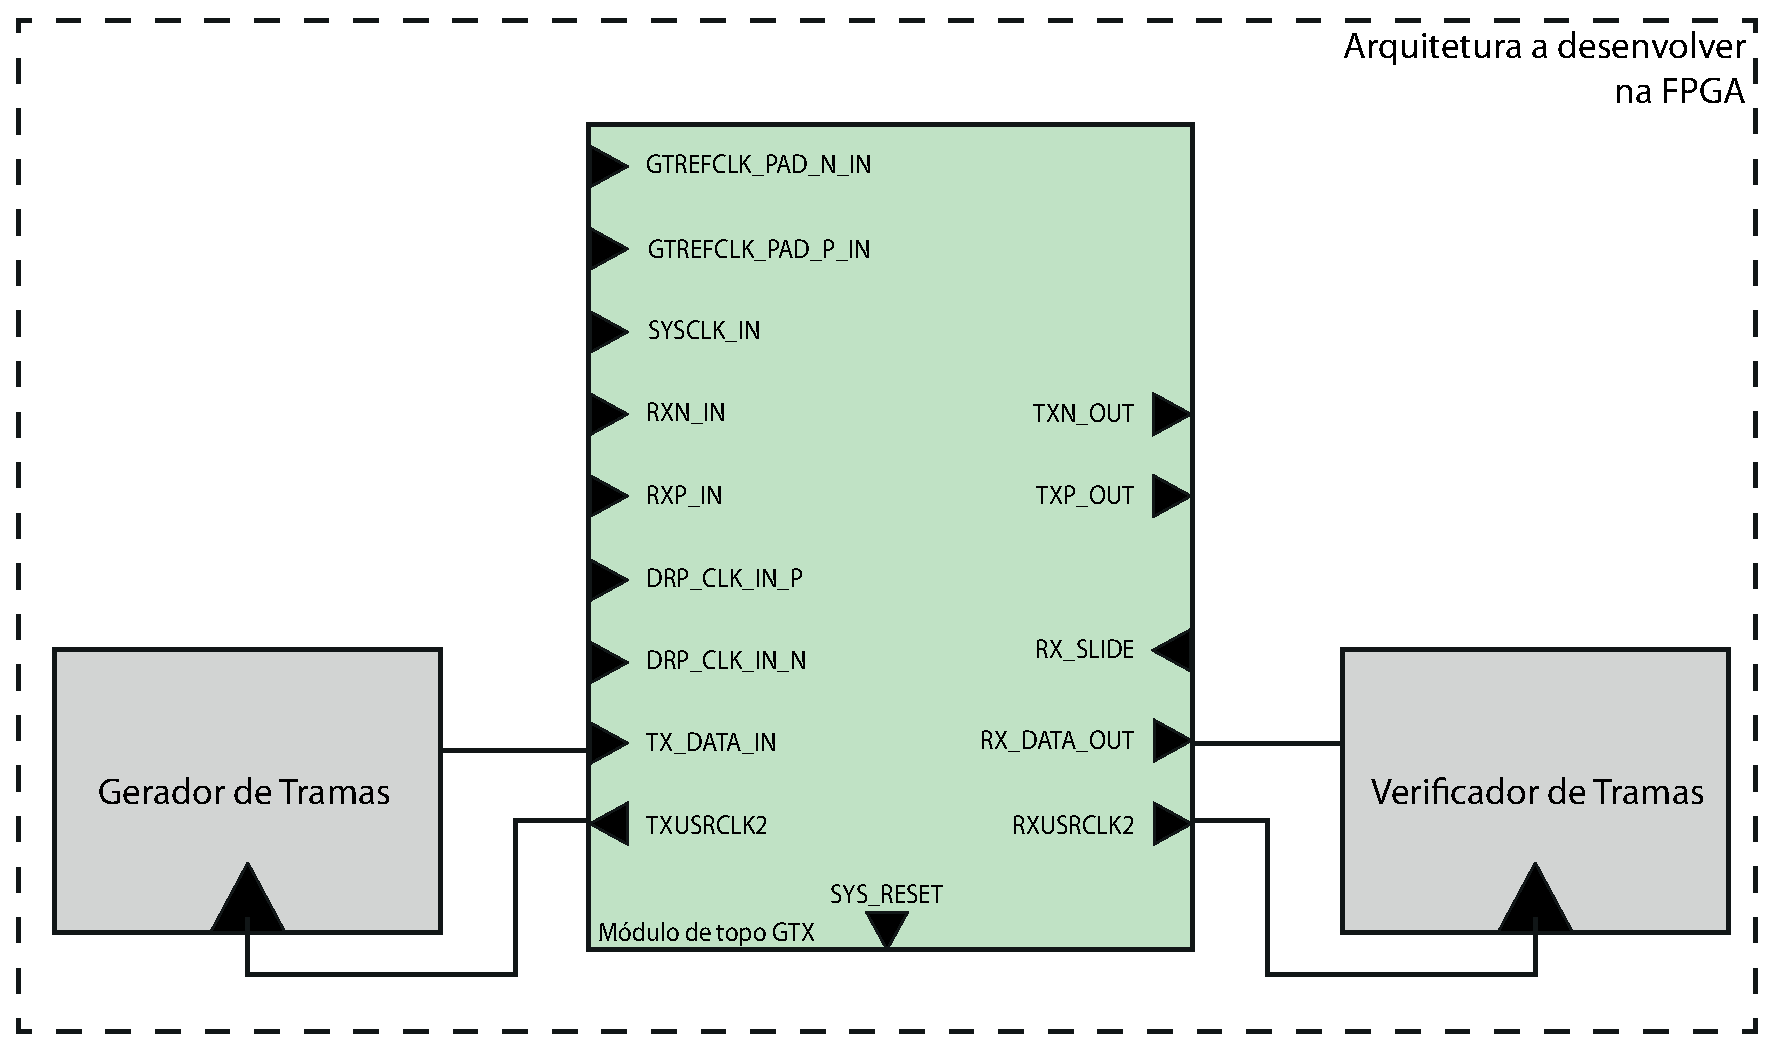
\includegraphics[width=1.0\textwidth]{gtx_wrapper}
		\captionsetup{width=1.0\linewidth}
		\caption[Estrutura geral do módulo GTX  gerado no \textit{software} VIVADO]{Estrutura geral do módulo GTX gerado no \textit{software} VIVADO}
		\label{fig:gtx_wrapper}
	\end{center}
\end{figure}

Na imagem \ref{fig:gtx_wrapper} da página  \pageref{fig:gtx_wrapper} visualiza-se a estrutura geral do IP GTX gerado pelo \textit{software} VIVADO. O módulo de topo representado na imagem é constituído por diversos sub-módulos, tal como indica o manual da interface que gera este IP referenciado em \cite{R022}. Contudo, esses sub-módulos são de gestão interna do transcetor e como tal não são relevantes para o projeto. Por esse motivo, nesta imagem apenas são apresentadas as portas de entrada e saída de maior importância para o projeto, que passam de seguida a ser detalhadas:

\begin{itemize}
	\item \textbf{GTREFCLK\_PAD\_N\_IN e GTREFCLK\_PAD\_P\_IN}:  Entrada do sinal de relógio diferencial externo de referência.
	
	\item \textbf{SYSCLK\_IN}: Entrada do sinal de relógio a que o resto da arquitetura opera, ou seja, o sinal de relógio de todos os outros blocos da arquitetura que não o GTX.
	
	\item \textbf{RXN\_IN e RXP\_IN}: Par diferencial de entrada do recetor  dos dados em série.
	
	\item \textbf{TXN\_OUT e TXP\_OUT}: Par diferencial de saída do transmissor dos dados em série.

	\item \textbf{DRP\_CLK\_IN\_P e DRP\_CLK\_IN\_N}: Entrada do par diferencial externo para a interface DRP (\textit{Dynamic Reconfiguration Port}). 
	
	\item \textbf{TX\_DATA\_IN}: Entrada dos dados em paralelo a serem serializados.
	
	\item \textbf{RX\_DATA\_OUT}: Saída dos dados em paralelo depois de recebidos e deserializados. 
	
	\item \textbf{TXUSRCLK2}: Sinal de relógio de amostragem dos dados para o transmissor.
	
	\item \textbf{RXUSRCLK2}: Sinal de relógio de amostragem dos dados provenientes do recetor.
	
	\item \textbf{RXSLIDE}: Entrada do sinal que ativa o alinhamento manual do recetor.
	
	\item \textbf{SYS\_RESET}: Sinal de \textit{reset} ativado pelas máquinas de estados do recetor e transmissor.
	
\end{itemize}
%%explicar que as portas que estão conectadas pq serao necessários aqueles blocos

Através da observação da imagem \ref{fig:gtx_wrapper} é possivel ver que a entrada TX\_DATA\_IN e a saída RX\_DATA\_OUT estão conectadas a dois blocos: um bloco gerador de tramas a enviar para o transmissor e um bloco que verifica as tramas que chegam do recetor. O funcionamento destes blocos pode variar de arquitetura para arquitetura, contudo em todas estes blocos operarão aos sinais de relógio TXUSRCLK2 e RXUSRCLK2 e são obrigatórios para o correto funcionamento do sistema globalmente.  Todos os outros sinais não estão diretamente conectados a nenhuma entrada nem saída porque podem variar entre as arquiteturas.

%%explicar o que é a interface DRP e q nao vai ser usada
A interface DRP é uma característica do transcetor que até agora não foi abordada porque não é utilizada no projeto. Esta interface permite configurar dinamicamente algumas características dos transcetores, o que é útil em alguns projetos. Apesar de não ser utilizada neste projeto, é impossível desativar esta característica na interface do \textit{software} que gera o módulo GTX, e por esse motivo está aqui brevemente apresentada.

%%explicar o porquê do RXSLIDE
É de notar ainda que a porta RXSLIDE apresentada na imagem \ref{fig:gtx_wrapper} da página \pageref{fig:gtx_wrapper} é uma porta que pode não existir se assim se pretender. Todavia optou-se por ativar estar porta pois é esta que ativa o alinhamento manual das palavras recebidas, e tal como mencionado em 
\ref{subsub:align} na página \pageref{subsub:align} deste mesmo capítulo, esta opção de alinhamento manual pode vir a ser útil para transmissões cuja taxa de é superior a 5 Gb/s. Através da análise da tabela \ref{table:line_rates} verifica-se que maior parte das taxas de débito calculadas para tramas com 32 bits ou mais são superiores a 5 Gb/s e como tal, é de esperar que tal venha a ser necessário.

%CONCLUIR_ESTA_SECÇÃO






%\section{Arquiteturas Desenvolvidas para a transmissão de dados em série}
%%%Dizer que para simplificar se fez isto isto e isto
%Nesta secção serão abordadas as arquiteturas desenvolvidas para a transmissão de dados em série, explicando todas as decisões tomadas para se obter o produto final. 
%
%\subsection{Abordagem inicial}
%
%Numa fase inicial do projeto optou-se por abordar de uma maneira simples a transmissão dos dados em série, sem o recurso à definição de todas a tramas do pacote a serem. Tal decisão foi tomada, ciente da importância das tramas num protocolo de comunicação, pois o IP GTX disponibilizado pela \textit{Xilinx} é muito complexo e completo e foi necessário uma familiarização com o mesmo.
%
%\subsubsection{Transmissão de uma barra de cores gerada na FPGA em série}
%
%A arquitetura desenvolvida in
%
%
%\subsubsection*{Concepção e Desenvolvimento}
%
%\subsubsection*{Resultados}









%\subsection{Definição de Tramas e Pacotes}
	
	
	
	
	
	
	
	
	%Em \cite{R031} é sugerido que o valor do sinal de relogio de referencia seja o mesmo proveninete da fonte HDMI isto porque a frequência o sinal de relógio de referência deve ser exatamente igual (ou multiplo) da cadência dos dados de entrada.